\documentclass[11pt]{article}
\usepackage{hyperref}
\usepackage{graphicx}
\usepackage[margin=2cm]{geometry}
\usepackage{amsmath}
\usepackage{booktabs}
\renewcommand{\Re}{\operatorname{Re}}
\renewcommand{\Im}{\operatorname{Im}}
\author{Shao-yu Tseng}
\date{\today}

\title{Homework \#5}
\begin{document}
\maketitle

\section{Magnetization vs Temperature}

From Figure \ref{fig:1}, we observe that the critical temperature is around 3.4, where the absolute magnetization abruptly drops to near zero. The temperature is scaled so that the transition probability is \(\exp(-\frac{\Delta E}{T})\) (i.e. \(k_B = 1\)). With fewer sweeps (hundreds to thousands), there appears to be some dips at temperatures below the critical value. I attribute them to random chance causing the spins to take longer to align at certain temperatures, as increasing the sweep count fixed it. Initially I was not able to get it to run fast enough, but I started using numba to produce JIT-compiled code that is much faster for the second part, which allowed it to run 200000 iterations in one minute (16 cores). The resources consulted are listed in the Contributions section.

\begin{figure}[htbp]
\label{fig:1}
\centerline{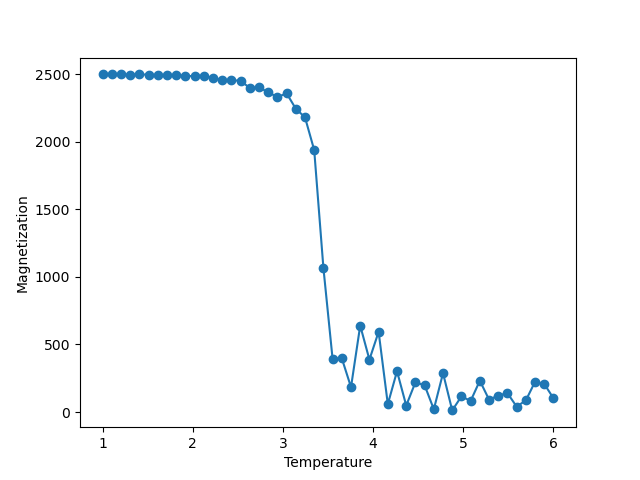
\includegraphics[width=0.7\textwidth]{ising-part1.png}}
\caption[]{M vs T}
\end{figure}
\pagebreak
\section{Max specific heat vs grid size}

From Figure \ref{fig:2}, in the center pane, we observe that the scaling law appears to hold for small values of n as the \(C_{\text{max}}\) curve has a similar shape to \(\log(n)\). In the left pane, we see that the peak of the specific heat lies close to the \(T_{C}\) determined in part 1. The \(C_{\text{max}}\) values are plotted again with a log scale x axis, which shows a nearly straight line, confirming this relation. This computation became extremely slow as the grid size and number of sweeps increases, even after using numba's JIT optimization to produce faster code (in the original python version, I could only run 200 sweeps, now I am running 100000, which was needed to get a decent result).

To be able to resume the computation after interruption, I implemented a way to save the results into files. I also observed some spurious spikes of specific heat at low temperatures that are single points. I applied a simple filter to remove the spikes from the data by interpolating neighboring results if the difference is too large. I suspect this is due to random chance and can be fixed with more iterations, but I cannot wait that long (this calculation already took an hour to run on 16 cores). For the same reason, I'm unable to extend the grid size to 500, as it would have taken too long. I added the data to the submission so you can run the script without waiting for the computation.

\begin{figure}[htbp]
\label{fig:2}
\centerline{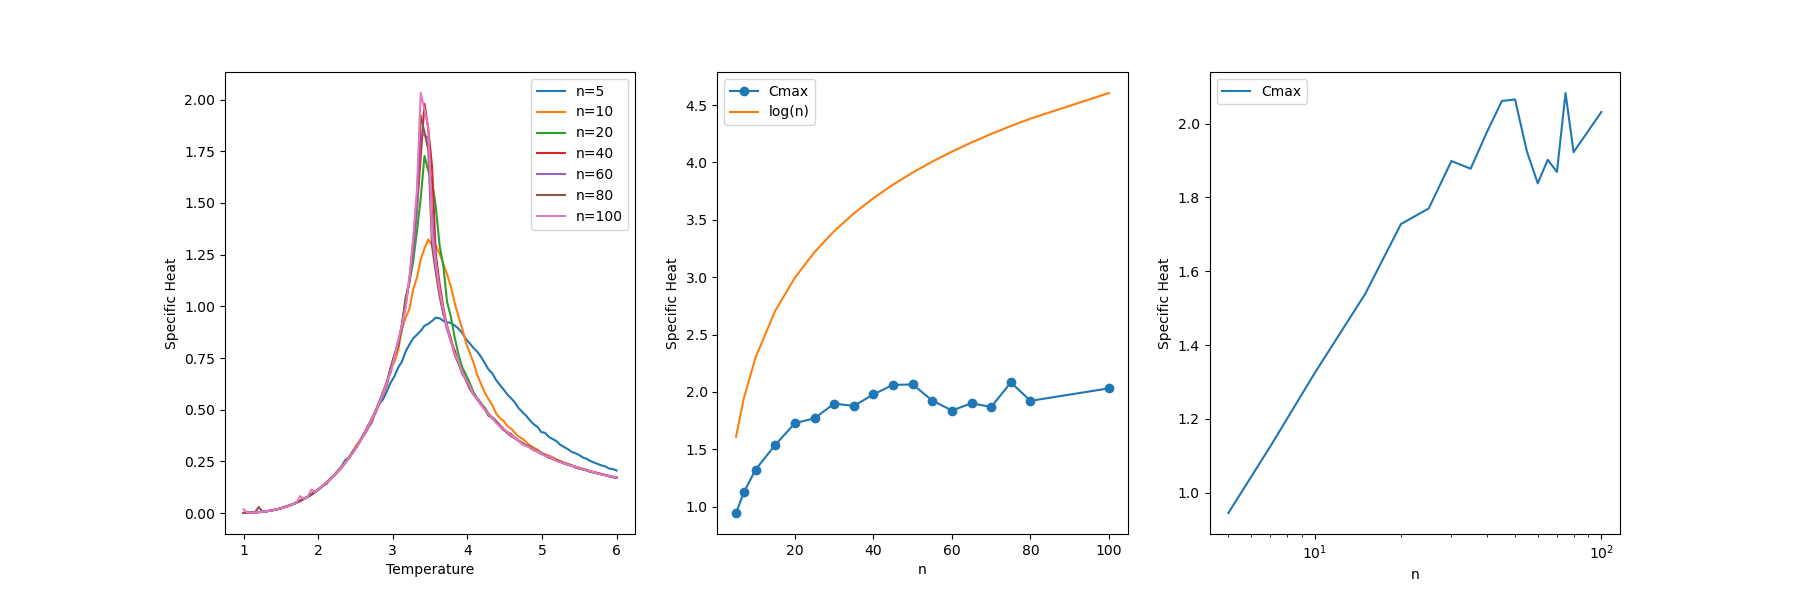
\includegraphics[width=\textwidth]{ising-part2.png}}
\caption[]{Max specific heat vs T and n}
\end{figure}
\pagebreak
\section{Contributions}
\subsection*{Metropolis algorithm description}

\url{https://phas.ubc.ca/~rozali/8.pdf}

\subsection*{Speeding up np.random operations (even this was too slow, eventually replaced by numba)}

\url{https://stackoverflow.com/questions/71940008/how-can-i-speed-up-the-mc-simulation-of-ising-model}

\subsection*{Python concurrent.futures (using multiple cores for speed up)}
\url{https://docs.python.org/3/library/concurrent.futures.html#concurrent.futures.ProcessPoolExecutor}

\subsection*{numba}
\url{https://numba.pydata.org/numba-doc/dev/reference/pysupported.html#supported-python-features}

This allows the code to run a lot faster without too much changes. Without this it would not be running nearly fast enough for so many iterations.

\subsection*{Critical temperature expression}
\url{https://sites.pitt.edu/~jdnorton/teaching/philphys/Ising_sim/index.html}

The critical temperature is 2.269 (with J = 1 \(k_B\)). Accounting for our J = 1.5 \(k_{B}\), the value would be 3.405. This helped with narrowing down the range of temperatures I need to plot.

\end{document}
